
%% bare_jrnl.tex
%% V1.4
%% 2012/12/27
%% by Michael Shell
%% see http://www.michaelshell.org/
%% for current contact information.
%%
%% This is a skeleton file demonstrating the use of IEEEtran.cls
%% (requires IEEEtran.cls version 1.8 or later) with an IEEE journal paper.
%%
%% Support sites:
%% http://www.michaelshell.org/tex/ieeetran/
%% http://www.ctan.org/tex-archive/macros/latex/contrib/IEEEtran/
%% and
%% http://www.ieee.org/



% *** Authors should verify (and, if needed, correct) their LaTeX system  ***
% *** with the testflow diagnostic prior to trusting their LaTeX platform ***
% *** with production work. IEEE's font choices can trigger bugs that do  ***
% *** not appear when using other class files.                            ***
% The testflow support page is at:
% http://www.michaelshell.org/tex/testflow/


%%*************************************************************************
%% Legal Notice:
%% This code is offered as-is without any warranty either expressed or
%% implied; without even the implied warranty of MERCHANTABILITY or
%% FITNESS FOR A PARTICULAR PURPOSE! 
%% User assumes all risk.
%% In no event shall IEEE or any contributor to this code be liable for
%% any damages or losses, including, but not limited to, incidental,
%% consequential, or any other damages, resulting from the use or misuse
%% of any information contained here.
%%
%% All comments are the opinions of their respective authors and are not
%% necessarily endorsed by the IEEE.
%%
%% This work is distributed under the LaTeX Project Public License (LPPL)
%% ( http://www.latex-project.org/ ) version 1.3, and may be freely used,
%% distributed and modified. A copy of the LPPL, version 1.3, is included
%% in the base LaTeX documentation of all distributions of LaTeX released
%% 2003/12/01 or later.
%% Retain all contribution notices and credits.
%% ** Modified files should be clearly indicated as such, including  **
%% ** renaming them and changing author support contact information. **
%%
%% File list of work: IEEEtran.cls, IEEEtran_HOWTO.pdf, bare_adv.tex,
%%                    bare_conf.tex, bare_jrnl.tex, bare_jrnl_compsoc.tex,
%%                    bare_jrnl_transmag.tex
%%*************************************************************************

% Note that the a4paper option is mainly intended so that authors in
% countries using A4 can easily print to A4 and see how their papers will
% look in print - the typesetting of the document will not typically be
% affected with changes in paper size (but the bottom and side margins will).
% Use the testflow package mentioned above to verify correct handling of
% both paper sizes by the user's LaTeX system.
%
% Also note that the "draftcls" or "draftclsnofoot", not "draft", option
% should be used if it is desired that the figures are to be displayed in
% draft mode.
%
\documentclass[journal]{IEEEtran}
\usepackage[utf8]{inputenc}
\usepackage[french]{babel}
\usepackage{graphicx} % graphics
\usepackage[style=numeric,citestyle=alphabetic,sorting=nty,backend=bibtex]{biblatex} 
\usepackage{amsmath}
\bibliography{whatmakeparis} 
%
% If IEEEtran.cls has not been installed into the LaTeX system files,
% manually specify the path to it like:
% \documentclass[journal]{../sty/IEEEtran}





% Some very useful LaTeX packages include:
% (uncomment the ones you want to load)


% *** MISC UTILITY PACKAGES ***
%
%\usepackage{ifpdf}
% Heiko Oberdiek's ifpdf.sty is very useful if you need conditional
% compilation based on whether the output is pdf or dvi.
% usage:
% \ifpdf
%   % pdf code
% \else
%   % dvi code
% \fi
% The latest version of ifpdf.sty can be obtained from:
% http://www.ctan.org/tex-archive/macros/latex/contrib/oberdiek/
% Also, note that IEEEtran.cls V1.7 and later provides a builtin
% \ifCLASSINFOpdf conditional that works the same way.
% When switching from latex to pdflatex and vice-versa, the compiler may
% have to be run twice to clear warning/error messages.






% *** CITATION PACKAGES ***
%
%\usepackage{cite}
% cite.sty was written by Donald Arseneau
% V1.6 and later of IEEEtran pre-defines the format of the cite.sty package
% \cite{} output to follow that of IEEE. Loading the cite package will
% result in citation numbers being automatically sorted and properly
% "compressed/ranged". e.g., [1], [9], [2], [7], [5], [6] without using
% cite.sty will become [1], [2], [5]--[7], [9] using cite.sty. cite.sty's
% \cite will automatically add leading space, if needed. Use cite.sty's
% noadjust option (cite.sty V3.8 and later) if you want to turn this off
% such as if a citation ever needs to be enclosed in parenthesis.
% cite.sty is already installed on most LaTeX systems. Be sure and use
% version 4.0 (2003-05-27) and later if using hyperref.sty. cite.sty does
% not currently provide for hyperlinked citations.
% The latest version can be obtained at:
% http://www.ctan.org/tex-archive/macros/latex/contrib/cite/
% The documentation is contained in the cite.sty file itself.






% *** GRAPHICS RELATED PACKAGES ***
%
\ifCLASSINFOpdf
  % \usepackage[pdftex]{graphicx}
  % declare the path(s) where your graphic files are
  % \graphicspath{{../pdf/}{../jpeg/}}
  % and their extensions so you won't have to specify these with
  % every instance of \includegraphics
  % \DeclareGraphicsExtensions{.pdf,.jpeg,.png}
\else
  % or other class option (dvipsone, dvipdf, if not using dvips). graphicx
  % will default to the driver specified in the system graphics.cfg if no
  % driver is specified.
  % \usepackage[dvips]{graphicx}
  % declare the path(s) where your graphic files are
  % \graphicspath{{../eps/}}
  % and their extensions so you won't have to specify these with
  % every instance of \includegraphics
  % \DeclareGraphicsExtensions{.eps}
\fi
% graphicx was written by David Carlisle and Sebastian Rahtz. It is
% required if you want graphics, photos, etc. graphicx.sty is already
% installed on most LaTeX systems. The latest version and documentation
% can be obtained at: 
% http://www.ctan.org/tex-archive/macros/latex/required/graphics/
% Another good source of documentation is "Using Imported Graphics in
% LaTeX2e" by Keith Reckdahl which can be found at:
% http://www.ctan.org/tex-archive/info/epslatex/
%
% latex, and pdflatex in dvi mode, support graphics in encapsulated
% postscript (.eps) format. pdflatex in pdf mode supports graphics
% in .pdf, .jpeg, .png and .mps (metapost) formats. Users should ensure
% that all non-photo figures use a vector format (.eps, .pdf, .mps) and
% not a bitmapped formats (.jpeg, .png). IEEE frowns on bitmapped formats
% which can result in "jaggedy"/blurry rendering of lines and letters as
% well as large increases in file sizes.
%
% You can find documentation about the pdfTeX application at:
% http://www.tug.org/applications/pdftex





% *** MATH PACKAGES ***
%
%\usepackage[cmex10]{amsmath}
% A popular package from the American Mathematical Society that provides
% many useful and powerful commands for dealing with mathematics. If using
% it, be sure to load this package with the cmex10 option to ensure that
% only type 1 fonts will utilized at all point sizes. Without this option,
% it is possible that some math symbols, particularly those within
% footnotes, will be rendered in bitmap form which will result in a
% document that can not be IEEE Xplore compliant!
%
% Also, note that the amsmath package sets \interdisplaylinepenalty to 10000
% thus preventing page breaks from occurring within multiline equations. Use:
%\interdisplaylinepenalty=2500
% after loading amsmath to restore such page breaks as IEEEtran.cls normally
% does. amsmath.sty is already installed on most LaTeX systems. The latest
% version and documentation can be obtained at:
% http://www.ctan.org/tex-archive/macros/latex/required/amslatex/math/





% *** SPECIALIZED LIST PACKAGES ***
%
%\usepackage{algorithmic}
% algorithmic.sty was written by Peter Williams and Rogerio Brito.
% This package provides an algorithmic environment fo describing algorithms.
% You can use the algorithmic environment in-text or within a figure
% environment to provide for a floating algorithm. Do NOT use the algorithm
% floating environment provided by algorithm.sty (by the same authors) or
% algorithm2e.sty (by Christophe Fiorio) as IEEE does not use dedicated
% algorithm float types and packages that provide these will not provide
% correct IEEE style captions. The latest version and documentation of
% algorithmic.sty can be obtained at:
% http://www.ctan.org/tex-archive/macros/latex/contrib/algorithms/
% There is also a support site at:
% http://algorithms.berlios.de/index.html
% Also of interest may be the (relatively newer and more customizable)
% algorithmicx.sty package by Szasz Janos:
% http://www.ctan.org/tex-archive/macros/latex/contrib/algorithmicx/




% *** ALIGNMENT PACKAGES ***
%
%\usepackage{array}
% Frank Mittelbach's and David Carlisle's array.sty patches and improves
% the standard LaTeX2e array and tabular environments to provide better
% appearance and additional user controls. As the default LaTeX2e table
% generation code is lacking to the point of almost being broken with
% respect to the quality of the end results, all users are strongly
% advised to use an enhanced (at the very least that provided by array.sty)
% set of table tools. array.sty is already installed on most systems. The
% latest version and documentation can be obtained at:
% http://www.ctan.org/tex-archive/macros/latex/required/tools/


% IEEEtran contains the IEEEeqnarray family of commands that can be used to
% generate multiline equations as well as matrices, tables, etc., of high
% quality.




% *** SUBFIGURE PACKAGES ***
%\ifCLASSOPTIONcompsoc
%  \usepackage[caption=false,font=normalsize,labelfont=sf,textfont=sf]{subfig}
%\else
%  \usepackage[caption=false,font=footnotesize]{subfig}
%\fi
% subfig.sty, written by Steven Douglas Cochran, is the modern replacement
% for subfigure.sty, the latter of which is no longer maintained and is
% incompatible with some LaTeX packages including fixltx2e. However,
% subfig.sty requires and automatically loads Axel Sommerfeldt's caption.sty
% which will override IEEEtran.cls' handling of captions and this will result
% in non-IEEE style figure/table captions. To prevent this problem, be sure
% and invoke subfig.sty's "caption=false" package option (available since
% subfig.sty version 1.3, 2005/06/28) as this is will preserve IEEEtran.cls
% handling of captions.
% Note that the Computer Society format requires a larger sans serif font
% than the serif footnote size font used in traditional IEEE formatting
% and thus the need to invoke different subfig.sty package options depending
% on whether compsoc mode has been enabled.
%
% The latest version and documentation of subfig.sty can be obtained at:
% http://www.ctan.org/tex-archive/macros/latex/contrib/subfig/




% *** FLOAT PACKAGES ***
%
%\usepackage{fixltx2e}
% fixltx2e, the successor to the earlier fix2col.sty, was written by
% Frank Mittelbach and David Carlisle. This package corrects a few problems
% in the LaTeX2e kernel, the most notable of which is that in current
% LaTeX2e releases, the ordering of single and double column floats is not
% guaranteed to be preserved. Thus, an unpatched LaTeX2e can allow a
% single column figure to be placed prior to an earlier double column
% figure. The latest version and documentation can be found at:
% http://www.ctan.org/tex-archive/macros/latex/base/


%\usepackage{stfloats}
% stfloats.sty was written by Sigitas Tolusis. This package gives LaTeX2e
% the ability to do double column floats at the bottom of the page as well
% as the top. (e.g., "\begin{figure*}[!b]" is not normally possible in
% LaTeX2e). It also provides a command:
%\fnbelowfloat
% to enable the placement of footnotes below bottom floats (the standard
% LaTeX2e kernel puts them above bottom floats). This is an invasive package
% which rewrites many portions of the LaTeX2e float routines. It may not work
% with other packages that modify the LaTeX2e float routines. The latest
% version and documentation can be obtained at:
% http://www.ctan.org/tex-archive/macros/latex/contrib/sttools/
% Do not use the stfloats baselinefloat ability as IEEE does not allow
% \baselineskip to stretch. Authors submitting work to the IEEE should note
% that IEEE rarely uses double column equations and that authors should try
% to avoid such use. Do not be tempted to use the cuted.sty or midfloat.sty
% packages (also by Sigitas Tolusis) as IEEE does not format its papers in
% such ways.
% Do not attempt to use stfloats with fixltx2e as they are incompatible.
% Instead, use Morten Hogholm'a dblfloatfix which combines the features
% of both fixltx2e and stfloats:
%
% \usepackage{dblfloatfix}
% The latest version can be found at:
% http://www.ctan.org/tex-archive/macros/latex/contrib/dblfloatfix/




%\ifCLASSOPTIONcaptionsoff
%  \usepackage[nomarkers]{endfloat}
% \let\MYoriglatexcaption\caption
% \renewcommand{\caption}[2][\relax]{\MYoriglatexcaption[#2]{#2}}
%\fi
% endfloat.sty was written by James Darrell McCauley, Jeff Goldberg and 
% Axel Sommerfeldt. This package may be useful when used in conjunction with 
% IEEEtran.cls'  captionsoff option. Some IEEE journals/societies require that
% submissions have lists of figures/tables at the end of the paper and that
% figures/tables without any captions are placed on a page by themselves at
% the end of the document. If needed, the draftcls IEEEtran class option or
% \CLASSINPUTbaselinestretch interface can be used to increase the line
% spacing as well. Be sure and use the nomarkers option of endfloat to
% prevent endfloat from "marking" where the figures would have been placed
% in the text. The two hack lines of code above are a slight modification of
% that suggested by in the endfloat docs (section 8.4.1) to ensure that
% the full captions always appear in the list of figures/tables - even if
% the user used the short optional argument of \caption[]{}.
% IEEE papers do not typically make use of \caption[]'s optional argument,
% so this should not be an issue. A similar trick can be used to disable
% captions of packages such as subfig.sty that lack options to turn off
% the subcaptions:
% For subfig.sty:
% \let\MYorigsubfloat\subfloat
% \renewcommand{\subfloat}[2][\relax]{\MYorigsubfloat[]{#2}}
% However, the above trick will not work if both optional arguments of
% the \subfloat command are used. Furthermore, there needs to be a
% description of each subfigure *somewhere* and endfloat does not add
% subfigure captions to its list of figures. Thus, the best approach is to
% avoid the use of subfigure captions (many IEEE journals avoid them anyway)
% and instead reference/explain all the subfigures within the main caption.
% The latest version of endfloat.sty and its documentation can obtained at:
% http://www.ctan.org/tex-archive/macros/latex/contrib/endfloat/
%
% The IEEEtran \ifCLASSOPTIONcaptionsoff conditional can also be used
% later in the document, say, to conditionally put the References on a 
% page by themselves.




% *** PDF, URL AND HYPERLINK PACKAGES ***
%
%\usepackage{url}
% url.sty was written by Donald Arseneau. It provides better support for
% handling and breaking URLs. url.sty is already installed on most LaTeX
% systems. The latest version and documentation can be obtained at:
% http://www.ctan.org/tex-archive/macros/latex/contrib/url/
% Basically, \url{my_url_here}.




% *** Do not adjust lengths that control margins, column widths, etc. ***
% *** Do not use packages that alter fonts (such as pslatex).         ***
% There should be no need to do such things with IEEEtran.cls V1.6 and later.
% (Unless specifically asked to do so by the journal or conference you plan
% to submit to, of course. )


% correct bad hyphenation here
\hyphenation{op-tical net-works semi-conduc-tor}


\begin{document}
%
% paper title
% can use linebreaks \\ within to get better formatting as desired
% Do not put math or special symbols in the title.
\title{Recherche bibliographie sur la reconnaissance des locations\\
		  \huge{à partir de l'article "What's make Paris look like Paris?"}}
%
%
% author names and IEEE memberships
% note positions of commas and nonbreaking spaces ( ~ ) LaTeX will not break
% a structure at a ~ so this keeps an author's name from being broken across
% two lines.
% use \thanks{} to gain access to the first footnote area
% a separate \thanks must be used for each paragraph as LaTeX2e's \thanks
% was not built to handle multiple paragraphs
%

\author{NGUYEN Van Tho,~\IEEEmembership{Promotion 17, Institut de la Francophonie pour 
l’Informatique}}

% note the % following the last \IEEEmembership and also \thanks - 
% these prevent an unwanted space from occurring between the last author name
% and the end of the author line. i.e., if you had this:
% 
% \author{....lastname \thanks{...} \thanks{...} }
%                     ^------------^------------^----Do not want these spaces!
%
% a space would be appended to the last name and could cause every name on that
% line to be shifted left slightly. This is one of those "LaTeX things". For
% instance, "\textbf{A} \textbf{B}" will typeset as "A B" not "AB". To get
% "AB" then you have to do: "\textbf{A}\textbf{B}"
% \thanks is no different in this regard, so shield the last } of each \thanks
% that ends a line with a % and do not let a space in before the next \thanks.
% Spaces after \IEEEmembership other than the last one are OK (and needed) as
% you are supposed to have spaces between the names. For what it is worth,
% this is a minor point as most people would not even notice if the said evil
% space somehow managed to creep in.



% The paper headers
\markboth{Bibliographie et étude de cas, Février~2014}%
{}
% The only time the second header will appear is for the odd numbered pages
% after the title page when using the twoside option.
% 
% *** Note that you probably will NOT want to include the author's ***
% *** name in the headers of peer review papers.                   ***
% You can use \ifCLASSOPTIONpeerreview for conditional compilation here if
% you desire.




% If you want to put a publisher's ID mark on the page you can do it like
% this:
%\IEEEpubid{0000--0000/00\$00.00~\copyright~2012 IEEE}
% Remember, if you use this you must call \IEEEpubidadjcol in the second
% column for its text to clear the IEEEpubid mark.



% use for special paper notices
%\IEEEspecialpapernotice{(Invited Paper)}




% make the title area
\maketitle

% As a general rule, do not put math, special symbols or citations
% in the abstract or keywords.
\begin{abstract}
Au cours des dernières années, l'émergence de médias géoréférencées, comme des photos 
géolocalisées, sur l'Internet a ouvert un tout nouveau monde de possibilités pour la 
recherche et les applications de la reconnaissance de locations. Cet axe de recherche 
est atteint beaucoup d'attention des chercheurs dans le domaine de traitement d'image et 
de vision par ordinateur. Ce rapport présente des recherches récentes sur la 
reconnaissance de la reconnaissance de locations en mettant l'accent sur les défis, les 
méthodes, les résultats atteints et les échelles de ces recherches.
\end{abstract}

% Note that keywords are not normally used for peerreview papers.
\begin{IEEEkeywords}
Traitement d'image, Vision par ordinateur, Reconnaissance des locations, Fouille de 
données
\end{IEEEkeywords}






% For peer review papers, you can put extra information on the cover
% page as needed:
% \ifCLASSOPTIONpeerreview
% \begin{center} \bfseries EDICS Category: 3-BBND \end{center}
% \fi
%
% For peerreview papers, this IEEEtran command inserts a page break and
% creates the second title. It will be ignored for other modes.
%\IEEEpeerreviewmaketitle



\section{Introduction}
\IEEEPARstart{C}{es} dernières années ont vu une explosion des données d'image sur 
Internet par une 
grande augmentation des images partagées sur les réseaux sociaux tels que Facebook et 
Flickr ou sur Google Street View. La reconnaissance des locations devient un besoin 
indispensable pour la recherche et la récupération d'images et est un domaine de 
recherche actif. La reconnaissance de locations partage des défis de la reconnaissance 
d'objets tels que la variation de point de vue, les différence d'échelle 
d'objet,le désordre du fond et l'occlusion. En plus de ces défis communs, la 
reconnaissance de locations a les difficultés de la grande taille de données et le manque 
des bases de données complètes. Plusieurs approches sont proposées pour résoudre ces
problèmes. Cependant, nous pouvons voir deux axes principaux: un pour la reconnaissance 
de locations à l'échelle globale \cite{Hays:2008:im2gps, gopalan2013learning} et un pour 
la reconnaissance de locations à petite échelle ( reconnaissance une location précise 
dans une ville, par exemple ) \cite{torii2013visual, sattler2012improving, cao2013graph}. 
Dans ce travail, nous présentons une petite revue sur les travaux récents de la 
reconnaissance de locations à l'échelle globale et à petite échelle. 

\section{Reconnaissance des locations à l'échelle globale}
Le but de la reconnaissance à cette échelle est pour répondre l'image requette est à 
partir de quelle région (ville ou pays). Une des caractéristiques de ce genre de problème 
est la base de données d'images de tout la planète. On peut résoudre le problème 
d'identification de location d'image \cite{Hays:2008:im2gps, gopalan2013learning} ou on 
peut résoudre un problème binaire: si l'image est d'une région \cite{doersch2012what}. 
Les défis de la reconnaissance de locations de cette échelle est d'abord la grande 
demande de calcul. De plus, en réalité, il est difficile de trouver une collection 
d'images qui peut couvrir tout la planète. %problème de GPS-marqués 

James Hays et al \cite{Hays:2008:im2gps} utilise un algorithme simple pour estimer la 
distribution de locations à partir d'une seule image en utilisant l'approche de 
la correspondance des scènes. Une base de données de 6 millions d'images GPS-marqués 
d'une collection en ligne Flickr est utilisée pour l'expérimentation. Dans ce travail, la 
position de l'image estimée est représentée comme une distribution de probabilité sur la 
surface de la Terre. Pour atteindre leur but, James Hays et al construisent une base de 
données en sélectionnant les images qui ont à la fois les coordonnées GPS et des 
mots-clés géographiques. Ceci augmente beaucoup la probabilité de trouver des données 
géolocalisées précisément et visuellement.

Pour trouver les correspondance des scènes, James Hays et al \cite{Hays:2008:im2gps} 
proposent une méthode qui utilise plusieurs types de caractéristiques: petite image à 
taille 16x16, histogramme en couleur CIE Lab, histogramme de texton, ligne de 
caractéristique, descripteur gist + couleur et contexte géométrique. %plus detaille ?
Les vecteurs caractéristiques sont pré-calculés pour toutes les images dans la base de 
données. Pour estimer location de l'image de requête, James Hays et al calcule d'abord le 
vecteur caractéristique pour cette image. Ce vecteur est ensuite comparé avec tous les 
vecteurs caractéristiques de base d'apprentissage. Plusieurs méthodes sont utilisées pour 
l'étape de reconnaissance: 1-NN, KNN sur les coordonnées GPS et clustering en utilisant 
Meanshift.

Le résultat d'expérimentation de James Hays et al afiché dans la figure \ref{fig:gps} 
montre que la méthode 1-NN 
et Meanshift rendent le résultat acceptable (avec un taux d'erreur de 25\%) à une échelle 
d'un petit pays. La méthode 1-NN fonctionne bien à petit échelle d'une ville alors que la 
méthode basant sur la méthode Meanshift est appropriée à l'échelle plus grande.
\begin{figure}[t]
    \centering
    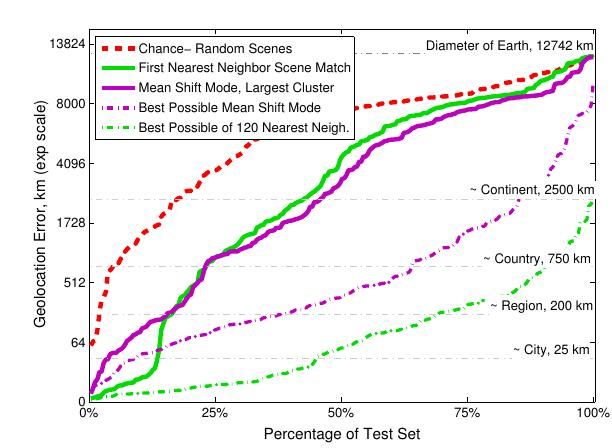
\includegraphics[width=9cm]{gps.jpg}
    \caption{ Précision de l'estimation de location} %caption here
    \label{fig:gps}
\end{figure}

\begin{figure}[t]
    \centering
    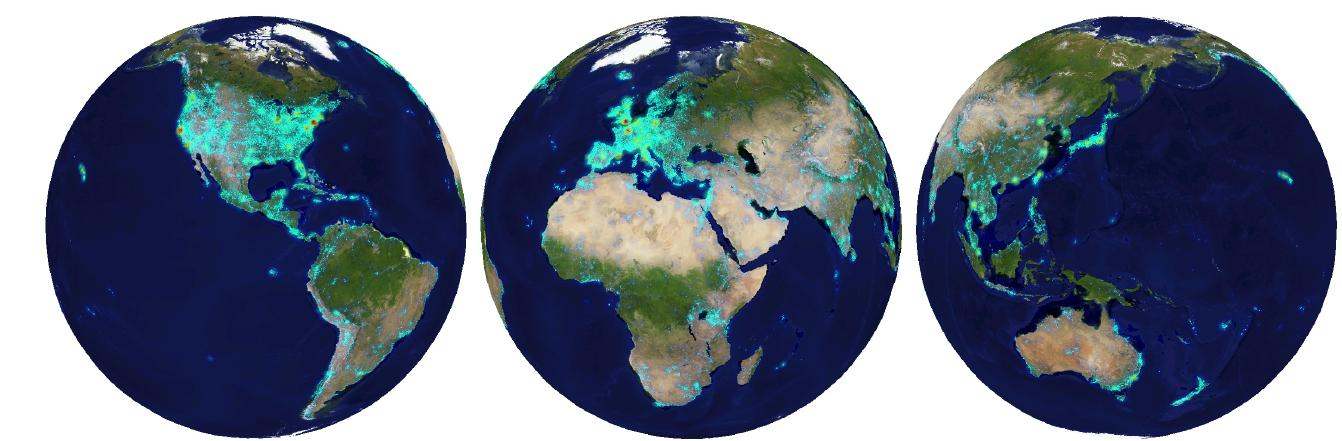
\includegraphics[width=9cm]{db.jpg}
    \caption{ Distribution d'images dans la base de données utilisée par James Hays et al 
\cite{Hays:2008:im2gps} et Raghuraman Gopalan \cite{gopalan2013learning}, location 
d'image est en cyan.}
    \label{fig:db}
\end{figure}

Utiliser la même base de données d'image que James Hays et al \cite{Hays:2008:im2gps}, 
Raghuraman Gopalan \cite{gopalan2013learning} cependant, utilise une approche de haut en 
bas. D'abord les domaines sont créés en regroupant les images des locations adjacentes, 
une hiérachie de domaines sont créée, un example de cette hiérachie est représenté dans 
la figure \ref{fig:hi}.
Les sous-espaces génératives et discriminatives aux domaines sont ensuite créés. Les 
informations cross-domain sont ensuite modèlisées en utilisant la géométrie de ces 
sous-espaces. Les images vont coder selon ces modèles pour inférer leur location. 

\begin{figure}[t]
    \centering
    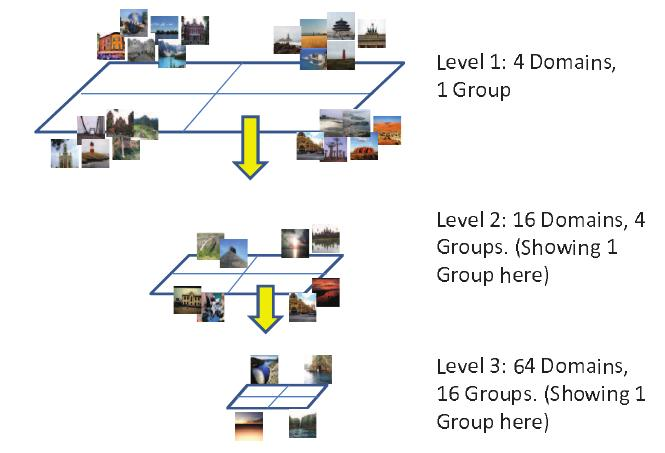
\includegraphics[width=8cm]{cr.jpg}
    \caption{Représentation d'une hiérachie des domaines}
    \label{fig:hi}
%caption here
\end{figure}

Un algorithme avec 4 étapes sont utilisé pour l'inférer la location d'image (figure 
\ref{fig:eta}). L'auteur expérimente son algorithme avec les differents nombres de 
caractéristiques. En utilisant toutes les caractéristiques, la performance de programme 
augmente. Dans cette revue, nous faisons attention à la performance de cette approche sur 
la base de données im2GPS. En fait, la performance de cette approche est meilleure que 
celle de James Hays et al \cite{Hays:2008:im2gps}. Ce résultat mets en accent 
l'importance de la modélisation de données sur le résultat. Cependant, nous constatons 
que cette approche n'est pas superieur à l'approche de James Hays et al 
\cite{Hays:2008:im2gps} en terme de scalabilité.

\begin{figure}[t]
    \centering
    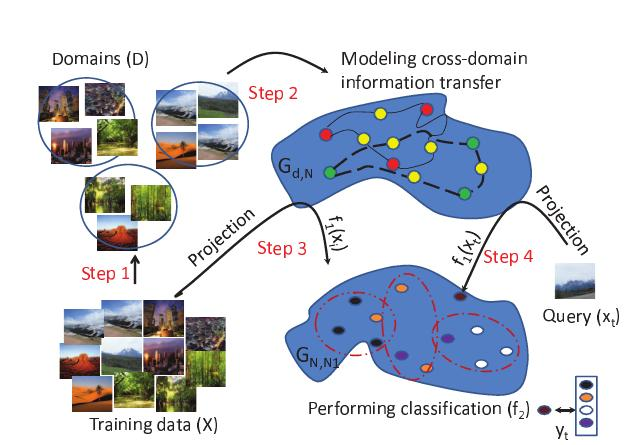
\includegraphics[width=8cm]{cr2.jpg}
    \caption{Les étapes pour inférer location d'images} %caption here
    \label{fig:eta}
\end{figure}
    
Le travail intitial de Carl Doersch et al \cite{doersch2012what} essaie  à chercher 
automatique des éléments visuels qui caractérisent une location géographique. Leur 
approche peut appliquer pour déterminer si l'image de requête est de la ville donnée. La 
base de données utilisée dans leur expérimentation est différence des autres. Ils ont 
choisi la base de données des images de Google Street Map qui offre certains avantages 
que les bases de données des résoudre sociaux tel que Flickr. 

Pour résoudre ce problème, les auteurs proposent une approche qui utilise la supervision 
géolocalisée et avec la construction des grappes de bas en haut.
On échantillonne aléatoirement un sous-ensemble de 25 000 parcelles à fort
contraste pour servir en tant que candidats pour l'ensemencement des grappes.
Les parcelles sont représentées en utilisant HOG [Dalal and
Triggs 2005]. Les candidates qui ont la plus proportion de ses voisins dans
l'ensemble négatif sont supprimés ainsi que les parcelles qui sont presque dupliquées
sont rejetées.
Pour améliorer le résultat, les auteurs appliquent itérativement un détecteur linaire SVM 
à chaque élément visuel. %3 étape

1) utilise k premiers voisins les plus proches dans l'ensemble positif comme des 
exemples positifs et toutes les parcelles dans l'ensemble négatif comme des exemples 
négatifs.

% Cela produit une petite amélioration
2)Dans cette étape, on réitère l'apprentissage SVM en utilisant 5 premières 
détections comme des exemples positifs.

3)On applique la validation croisée en divisant les deux parties positive et 
négative de données en l sous-ensembles à même taille. À chaque itération de 
l'apprentissage, on applique les détecteurs formés dans l'étape précédente à un 
nouveau sous-ensemble de données pour sélectionner les k détections pour 
rapprendre. Des centaines des détecteurs vont choisir comme les éléments 
visuels géo-informatives.\\

Pour évaluer les éléments visuels, Carl Doersch et al testent une nouvelle données dont 
50\% images de Paris et 50\% d'ailleurs en utilisant les 100 premiers détecteurs de
Paris. La précision des meilleurs détecteurs était 83\%. Pour Prague ce taux
était 92\%. Alors que les résultats des volontaires étaient 78.5 \%. Ce résultat est très 
prometteur. Cependant, les résultats de l'algorithme sur les villes américaines sont très 
limites car les styles aux États-Unis manquent des cohérences et des originalités. 
D'autre limite de cette approche est qu'il est appliqué seulement aux régions urbains, 
quand on veut l'appliquer sur des scènes naturelles telles que des forêts, des montages 
... les éléments visuels sont très peu discriminatifs. 


\section{Reconnaissance des locations à petit échelle}
Étant donné une base de données d'images d'une ville, la tâche de la reconnaissance de 
locations est de trouver la location exacte de l'image de requête. Les méthodes proposées 
récemment sont basées sur la méthode "Sac de mots" avec des modifications et 
des extensions \cite{torii2013visual, sattler2012improving, cao2013graph}.

Akihiko Torii et al \cite{torii2013visual} propose une méthode pour la reconnaissance des 
locations avec les structures répétitives. Leur motivation est qu'en réalité, les 
structures répétitives ( qui sont ignorés dans la méthode "Sac de mots visuels") peuvent 
porter des informations importantes. Ils visent à utiliser ces structures 
pour améliorer la reconnaissance de location de la méthode Sac de mots visuels. Au lieu 
d'être supprimés, les structures répétitives sont détectées et ajustées leurs poids. 

Pour détecter les répétitives, un graphe $G=(V,E)$,  $E=\{(x_i, s_i, d_i)\}$ est 
construit avec $x_i$ est local invariant features, $s_i$ est la facteur d'échelle et  
$d_i$ est la descripteur SIFT. Chaque descripteur SIFT est en outre affecté au K = 
50 mots visuels les plus proches d'un vocabulaire visuel pré-calculée. Les sommets $V_i$ 
et $V_j$ sont connexe si 1) $||x_i-x_j|| < c (s_i + s_j)$; c=10, 2) deux caractéristiques 
ont au moins un mot visuel en commun, 3) la ratio d'échelle $\sigma$ est entre 0.5 et 
1.5. Les groupes des caractéristiques sont construits en trouvant les composantes 
connexes du graphe. Les auteurs visent à représenter la présence des répétitions plus que 
le nombre de correspondances d'éléments répétitifs.Une image est représentée par 
un vecteur:
\begin{center}
	   $r_d=(r_1, r_2, \dots, r_V)^T$
\end{center}
  ou le i-ème mot visuel pèse:
\begin{center}
\begin{equation}
r_i=\begin{cases} 
	w_{id} \ si \  w_{id} > 0\ et\ w_{id} < T \\
	T\ si\ w_{id} > T
	\end{cases}
\end{equation}

\end{center}
La constance T est pour but de représenter l'occurrence ( présence / absence ) du mot 
visuel , plutôt que de mesurer le nombre réel d'occurrences. 
Le poids $w_{id}$ du mot visuel i-ème dans l'image d est obtenue en agrégeant le poids 
adaptative doux attribué à travers l'image en tenant compte les structures répétitives. 
Ceci est plus précis et moins ambigu que ceux dans l'état de l'art. 
Pour vérifier l'algorithme proposée, Akihiko Torii et al \cite{torii2013visual} 
l'expérimentent avec une base de données d'image de Google Street View de la ville 
Pittsburgh et de la ville San Francisco. Le résultat montre que les structures 
répétitives améliorent le taux de rappel ( figure 5 ).
%resultat
\begin{figure}[t]
    \centering
    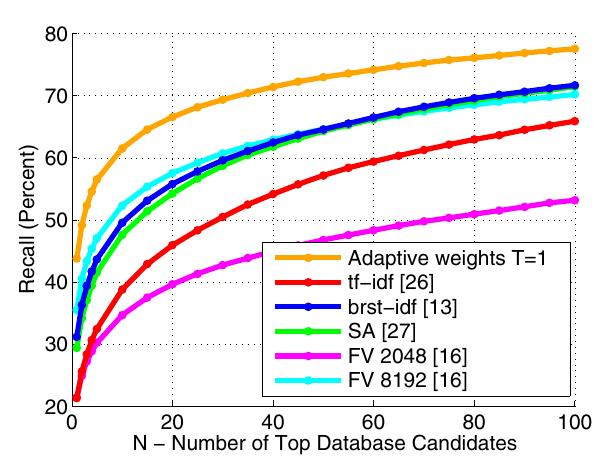
\includegraphics[width=8cm]{ad.jpg}
    \label{fig:add}
    \caption{Taux de rappel sur la base de données Pittsburgh, résultat de 
\cite{torii2013visual} est en jaune} %caption hereEvaluation on \end{figure}
\end{figure}

Song Cao et Noah Snavely \cite{cao2013graph} mettent en accent la représentation de la
données. Leur exploitation montre que une représentation de base de données en graphe 
améliore la performance de la reconnaissance de location d'une méthode basant sur la 
méthode Sac de mots visuels. L'approche de ce travail basant directement sur la méthode 
Sac de mots visuels dont les images sont représentées comme le L2 normalisé de 
histogramme 
des mots visuels. En plus des vecteurs de sac de mots, un graphe des images sont aussi 
utilisé dont chaque noeuds est une image et les sommets représentent les chevauchements 
entre les images (figure 6).  
\begin{figure}[t]
    \centering
	  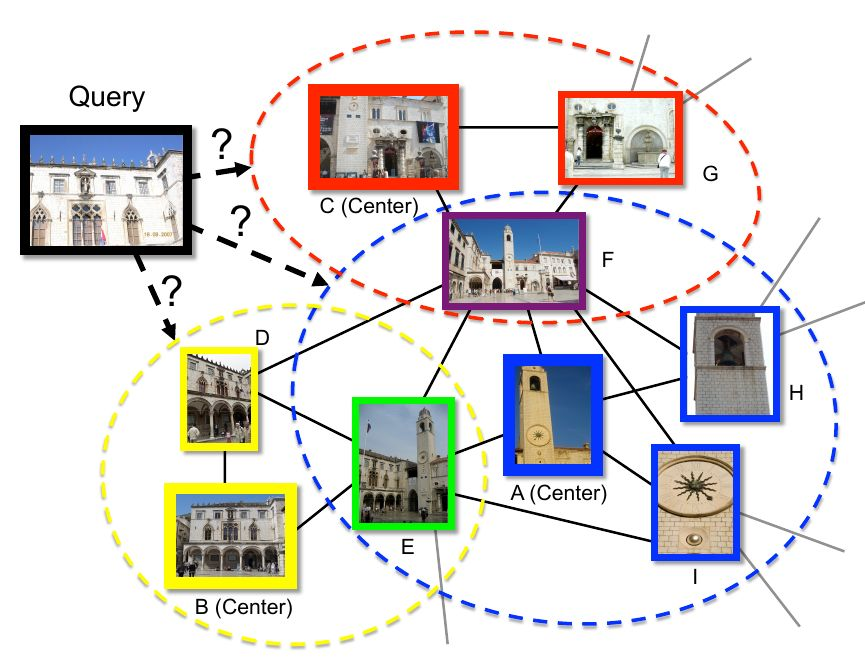
\includegraphics[width=7cm]{gra1.jpg}
    \label{fig:grp}
    \caption{Un segment d'un graphe avec 3 clusters définis par les images A, B, C} 
\end{figure}

L'idée principale de cette méthode est d'abord récuper des images similaires (short 
list) dans la base de données et ensuite mettre en correspondance détaillée jusqu'à une 
correspondance est trouvée. À étape d'apprentissage, une fonction de similarité est 
appliquée sur les sous-graphes. Ces sous-graphes sont créés en utilisant un algorithme 
glouton qui permet d'éviter un problème NP-Complet. À étape de reconnaissance, la 
distance entre l'image de requête et chaque image de base d'apprentissage, une liste des 
images similaires est générée. En suite, une vérification géométrique est réalisée avec 
les meilleurs images dans la liste des images similaires. Les auteurs proposent aussi 
quelques méthodes pour améliorer la qualité de la liste des images similaires (short 
list). 
L'algorithme peut atteindre un taux de précision de 99.5\% sur la base de données de 
Dubrovnik et 99.7\% sur la base de données de Rome. Ces taux de précision sont meilleurs 
que ceux de la méthode Sac de mots qui sont 98.5\% et 99.6\%.

Cette méthode rend des résultats meilleurs que ceux de la méthode Sac de mots. Cependant, 
son implémentation est complexe et besoin plus de mémoire.

Torsten Sattler, Bastian Leibe et Leif Kobbelt \cite{sattler2012improving} proposent une 
recherche active basant sur les deux recherches de 2D à 3D et de 3D à 2D pour les 
correspondances supplimantaires. Les descripteurs des caractéristiques 2D et des points 
3D sont assignés aux mots visuels (figure \ref{fig:aat}). La pose de caméra est estimée 
en 
utilisant l'algorithme RANSAC. Ces correspondances 2D-3D déclenchent un processus de 
mettre en correspondance 
3D-2D. Cette nouvelle approche a la même performance que la méthode basant sur 
l'arbre mais beaucoup plus rapide. L'idée de la recherche active est qu'après avoir 
trouvé une correspondance 2D-3D, on cherche activement $N_{3D}$ points plus proches 
à cette correspondance. %more detail

\begin{figure}[t]
    \centering
	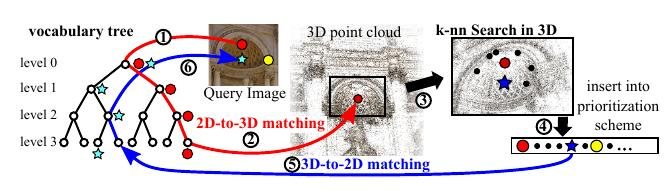
\includegraphics[width=9cm]{at.jpg}
    \caption{Description de la méthode recherche active} %caption here
    \label{fig:aat}
\end{figure}

En comparaison le résultat de cette méthode aux ceux dans littérature, on constate 
qu'elle peut rendre des meilleurs résultats en gardant plus de correspondances qui ont 
perdu à cause de la quantification. De plus, l'objectif des auteurs sont atteint quand 
la vitesse leur algorithme est comparable aux autres algorithmes.

\section{Conclusion}
La reconnaissance de location est un thème de recherche très actif grâce à l'exposition 
de sources d'images sur Internet. Dans ce travail, nous présentons des recherches sur la 
reconnaissance de location de ces dernières années pour mettre l'accent sur les résultats 
atteints et les défis à différentes échelles.
\nocite{*}
\printbibliography
\end{document}